% 2021 新高考Ⅱ卷 10：四个正方体选项图 (A)(B)(C)(D)
% 绘制依据：源 PDF（deekur/gaokaomath 2021新高考2）第 1 页原图，经 260dpi 裁剪逐图核对点位。
% 统一设棱长 2：前面正方形 (0,0)-(2,2)，后向偏移 (0.85,0.5)；O 为下底面中心。
% 画布坐标 = (x + 0.425y, z + 0.25y)，立体坐标系：x 右、y 后、z 上。
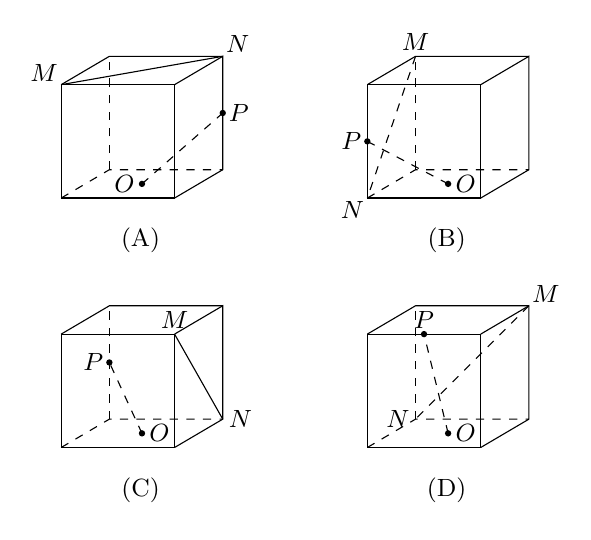
\begin{tikzpicture}[scale=0.72, font=\small]
  % ---------- (A)：M(0,0,2) 左前上，N(2,2,2) 右后上，P(2,2,1) 右后竖棱中点；MN 上底面对角线 ----------
  \begin{scope}
    \draw (0,0) rectangle (2,2);
    \draw (2,0) -- (2.85,0.5) -- (2.85,2.5) -- (2,2);
    \draw (0,2) -- (0.85,2.5) -- (2.85,2.5);
    \draw[dashed] (0,0) -- (0.85,0.5) -- (2.85,0.5);
    \draw[dashed] (0.85,0.5) -- (0.85,2.5);
    \coordinate (M) at (0,2);      \coordinate (N) at (2.85,2.5);
    \coordinate (P) at (2.85,1.5); \coordinate (O) at (1.425,0.25);
    \draw (M) -- (N);
    \draw[dashed] (O) -- (P);
    \fill (P) circle (1.6pt); \fill (O) circle (1.6pt);
    \node[above left, inner sep=1pt] at (M) {$M$};
    \node[above right, inner sep=1pt] at (N) {$N$};
    \node[right, inner sep=2pt] at (P) {$P$};
    \node[left, inner sep=2.5pt] at (O) {$O$};
    \node at (1.4,-0.75) {(A)};
  \end{scope}
  % ---------- (B)：M(0,2,2) 左后上，N(0,0,0) 左前下，P(0,0,1) 左前竖棱中点；MN 左侧面对角线（被遮挡） ----------
  \begin{scope}[xshift=5.4cm]
    \draw (0,0) rectangle (2,2);
    \draw (2,0) -- (2.85,0.5) -- (2.85,2.5) -- (2,2);
    \draw (0,2) -- (0.85,2.5) -- (2.85,2.5);
    \draw[dashed] (0,0) -- (0.85,0.5) -- (2.85,0.5);
    \draw[dashed] (0.85,0.5) -- (0.85,2.5);
    \coordinate (M) at (0.85,2.5); \coordinate (N) at (0,0);
    \coordinate (P) at (0,1);      \coordinate (O) at (1.425,0.25);
    \draw[dashed] (M) -- (N);
    \draw[dashed] (O) -- (P);
    \fill (P) circle (1.6pt); \fill (O) circle (1.6pt);
    \node[above, inner sep=2pt] at (M) {$M$};
    \node[below left, inner sep=1pt] at (N) {$N$};
    \node[left, inner sep=2pt] at (P) {$P$};
    \node[right, inner sep=2.5pt] at (O) {$O$};
    \node at (1.4,-0.75) {(B)};
  \end{scope}
  % ---------- (C)：M(2,0,2) 右前上，N(2,2,0) 右后下，P(0,2,1) 左后竖棱（隐藏棱）中点；MN 右侧面对角线 ----------
  \begin{scope}[yshift=-4.4cm]
    \draw (0,0) rectangle (2,2);
    \draw (2,0) -- (2.85,0.5) -- (2.85,2.5) -- (2,2);
    \draw (0,2) -- (0.85,2.5) -- (2.85,2.5);
    \draw[dashed] (0,0) -- (0.85,0.5) -- (2.85,0.5);
    \draw[dashed] (0.85,0.5) -- (0.85,2.5);
    \coordinate (M) at (2,2);      \coordinate (N) at (2.85,0.5);
    \coordinate (P) at (0.85,1.5); \coordinate (O) at (1.425,0.25);
    \draw (M) -- (N);
    \draw[dashed] (O) -- (P);
    \fill (P) circle (1.6pt); \fill (O) circle (1.6pt);
    \node[above, inner sep=2pt] at (M) {$M$};
    \node[right, inner sep=2pt] at (N) {$N$};
    \node[left, inner sep=2pt] at (P) {$P$};
    \node[right, inner sep=2.5pt] at (O) {$O$};
    \node at (1.4,-0.75) {(C)};
  \end{scope}
  % ---------- (D)：M(2,2,2) 右后上，N(0,2,0) 左后下，P(1,0,2) 前上棱中点；MN 后侧面对角线（被遮挡） ----------
  \begin{scope}[xshift=5.4cm, yshift=-4.4cm]
    \draw (0,0) rectangle (2,2);
    \draw (2,0) -- (2.85,0.5) -- (2.85,2.5) -- (2,2);
    \draw (0,2) -- (0.85,2.5) -- (2.85,2.5);
    \draw[dashed] (0,0) -- (0.85,0.5) -- (2.85,0.5);
    \draw[dashed] (0.85,0.5) -- (0.85,2.5);
    \coordinate (M) at (2.85,2.5); \coordinate (N) at (0.85,0.5);
    \coordinate (P) at (1,2);      \coordinate (O) at (1.425,0.25);
    \draw[dashed] (M) -- (N);
    \draw[dashed] (O) -- (P);
    \fill (P) circle (1.6pt); \fill (O) circle (1.6pt);
    \node[above right, inner sep=1pt] at (M) {$M$};
    \node[left, inner sep=2pt] at (N) {$N$};
    \node[above, inner sep=2pt] at (P) {$P$};
    \node[right, inner sep=2.5pt] at (O) {$O$};
    \node at (1.4,-0.75) {(D)};
  \end{scope}
\end{tikzpicture}